\begin{wrapfigure}{R}{0.2\textwidth}
    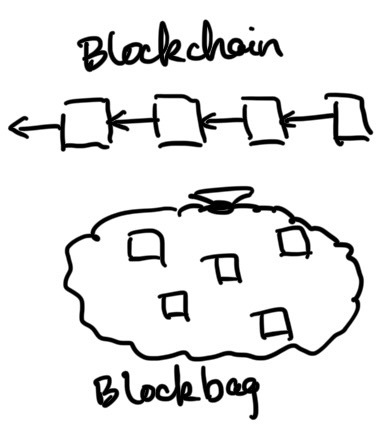
\includegraphics[width=0.2\textwidth]{graphs/IMG_0066}
\end{wrapfigure}

\paragraph{The only-for-finality mechanism.}
The \emph{chain} structure in blockchains corresponds to its inherent ordering functionality.
To clearly draw the difference between them and the finality mechanism in \sys, we explicitly change the representation from ``a chain of blocks'' to ``a (unordered) set of blocks''.
\sgd{Or ``a bag of blocks'' if that is more vivid.}
\sgd{Blockbag? :)}

The \emph{append-only} property of blockchains is expected to be preserved, though.
Anything (or any block) that has been finalized is expected to not get ``de-finalized'' indefinitely.
This property directly enables blockchains to execute the blocks in the finalization order, and \sys also relies on it.
The ``append'' here seems to imply the ordered direction.
Since our finality is unordered, maybe should call it \emph{insert-only}, while the logical clocks are the ones that append-only, to draw a clear distinction.

Since the finality mechanism in \sys requires a subset of blockchains functionalities, blockchains can certainly serve as the finality mechanism.
If necessary we may conduct research on alternative finality mechanisms, but blockchains, especially Ethereum, are probably good enough for now.

\paragraph{What is getting ordered?}
In blockchains it's ``blocks'' that are getting ordered, and inside the blocks it's ``transactions'' that are ordered (subjectively) by the blocks' proposers.
The two-layer design is purely for performance optimization (\ie batching) and has no practical meaning, to we can ignore the outer layer and simply say it's transactions that are getting ordered.

The meaning of \emph{transaction}, though heavily overloaded, probably implies finality.
In \sys what get ordered has no finality (yet).
It is only finalized when it has been submitted to the finality mechanism, not upon ordered.
In another word, they are not transactions ``yet'' upon ordered, and they may or may not ``turn into'' transactions depending on whether they will eventually be finalized.

In the logical clock related introductions we usually put it as it's ``events'' that get ordered.
Since we are describing a financial market solution here I would realize the concept as \emph{quotes}, \emph{preorders} or \emph{letters of intent}, and \emph{intents} to refer them as a whole.
It's probably fine to reuse \emph{transaction} to refer what has been submitted for finality.

\paragraph{The properties of ordering.}
\sgd{If necessary (which probably is), discuss the rationale behind these properties.
What bad things can happen if we don't have them?}
\begin{itemize}
    \item Share-nothing distributed.
    The ordering mechanism itself does not require propagation \ie communication across the whole system.
    In another word, \sys does not forcefully \emph{push} the ordered intents, like how blockchains push the ordered blocks, to the nodes.
    Nodes certainly need to actively \emph{pull} the intents that are involved in the orders they would propose, and that is on demand.
    The system shares nothing more than the minimum.
    \sgd{In previous discussions this has been referred as ``laziness'' or ``lazy consensus''.
    Those words are also not bad in precision, and we can use them if they are better marketing terms.}
    
    \item Optimal parallelization, this is closely related to the previous.
    More than one node can contribute to the ordering concurrently/simultaneously, and if necessary every node can contribute at the same time.
    This is completely on the opposite to the blockchains, where \emph{at most one} node can contribute to the ordering at any time \ie the qualified proposer of the round.

    No matter when, no matter where, no matter whom in the \sys system wants to order no matter what, they can do it \emph{immediately}, without waiting for anything \eg becoming the proposers.
    
    \item Verifiable and append-only.
    These are the revisiting properties of blockchains.
    They are necessary to \emph{preserve} the finality through all ordered intents.
    The following explains this more in action.
\end{itemize}

\begin{wrapfigure}{R}{0.4\textwidth}
    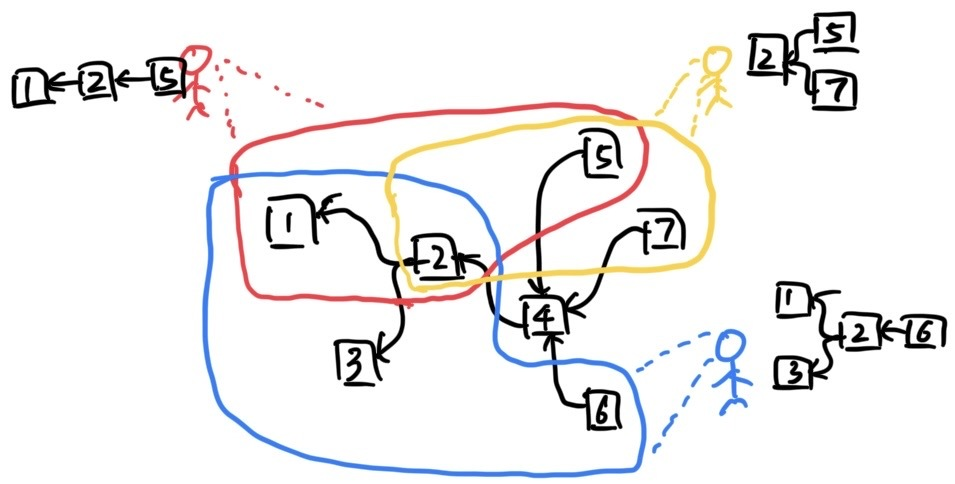
\includegraphics[width=0.4\textwidth]{graphs/IMG_0064}
\end{wrapfigure}

\paragraph{The cooperation.}
The ordering mechanism forms a \emph{partial ordering} among the intents.
Notice that although we represent the partial ordering as a single graph in the illustration, the graph is not shared in reality.
In another word, (probably) no one in \sys actually get to know the whole graph.
Everyone can only learn it partially, according to their point of view.

However, everyone's partial view is guaranteed to be \emph{compatible} to the other's one.
Every partial view is a subgraph of the whole graph.
And if you merge all subgraphs together, you just get the whole graph back, without any risk of confliction.
\sgd{Well, these material may be a bit too technical, try rephrase it more comprehensively.}

\begin{figure}[H]
    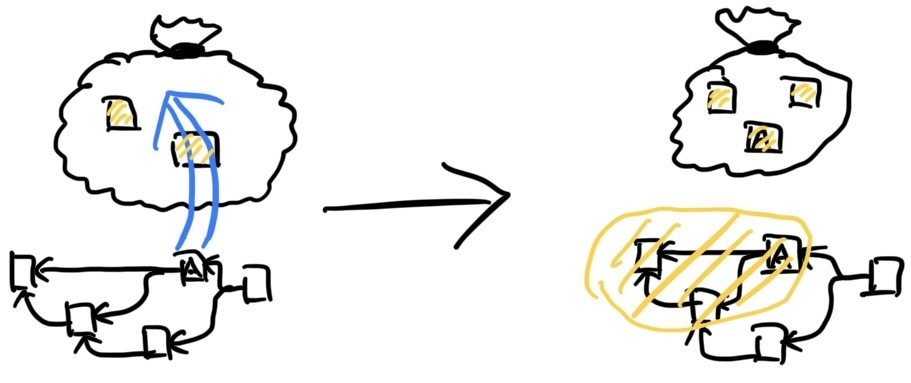
\includegraphics[width=0.5\textwidth]{graphs/IMG_0065}
    \Description{}
\end{figure}

If anyone wants to finalize an intent \ie ``make a deal'' according to it, they submit the intent to finality.
As we stated above, finality mechanism in \sys is an insert-only bag of intents.
Effectively, the finality mechanism \emph{endorses} the intents by inserting them into the consensus bag.
The transitivity of \sys's partial ordering extends the \emph{endorsement} to a larger set of intents.
\sgd{This happens to match the \emph{transitivity closure} concept in mathematic.
(Well, not completely accidentally, I have designed it in this way.)
Make use of this fact if having a proper formalization helps in some way.}

What important is that the extended endorsement is \emph{finalized}.
Although finality mechanism does not explicitly finalize every endorsed intents, it is safe to consider all of them finalized, thanks to the verifiable and append-only properties of the ordering mechanism.
As the result, \sys's ordering mechanism becomes an \emph{amplifier} for finality.
\sys not only enables real time ordering, but also \emph{more} finality.
We believe that nodes can only be incentivized to propose ordered intents that will be finalized (probabilistically), just like they can only be incentivized to propose blocks if the blocks will be chained.
With our ordering mechanism design, the fact that the ordering is not happening inside finality mechanism doesn't change the fact that the ordering still can be finalized, so \sys does not expose challenges in economics.

\sgd{Weird material above, probably fits somewhere else.}

Intents do conflict.
That's why finality does not endorse every submitted intent, but only the \emph{compatible} ones.
What intents are compatible is application specific, which is a topic elaborated in the following section.
In the worst case, intents that do not reside on the same chain all conflict to each other.
Those are the applications that essentially make use of shared mutable states, and they would better directly deploy on blockchains.
We expect our targeted applications to have few contentions on the finality, but every finality involves a lot of collaboration efforts, and the willingness of the collaborations all come with \emph{preconditions}, or assumptions.
This sounds a lot abstract, but as shown below, finance can be one such case.

\sgd{Personally I'm already satisfied by describing ``what we are good for'' in one sentence, regardless of the abstractness.}